\documentclass[aspectratio=169,11pt]{beamer}

% -----------------------------------------------------------------------------
% Self-contained presentation setup
% -----------------------------------------------------------------------------
\usepackage[T1]{fontenc}
\usepackage{lmodern}
\usepackage{amsmath,amssymb,mathtools}
\usepackage{booktabs}
\usepackage{tabularx}
\usepackage{listings}
\usepackage{tikz}
\usepackage[most]{tcolorbox}
\usepackage{appendixnumberbeamer}
\usetikzlibrary{arrows.meta,calc,fit,matrix,positioning,shapes.geometric}

\usetheme{Boadilla}
\usecolortheme{seagull}
\setbeamertemplate{navigation symbols}{}
\setbeamertemplate{items}[circle]
\setbeamertemplate{enumerate items}[default]
\setbeameroption{hide notes}

\definecolor{osblue}{RGB}{28,86,145}
\definecolor{osgreen}{RGB}{36,125,91}
\definecolor{osorange}{RGB}{202,105,36}
\definecolor{osred}{RGB}{166,45,45}
\definecolor{osgray}{RGB}{74,85,104}
\setbeamercolor{structure}{fg=osblue}
\setbeamercolor{alerted text}{fg=osred}
\setbeamercolor{block title}{bg=osblue!15,fg=black}
\setbeamercolor{block body}{bg=osblue!4,fg=black}

\newcommand{\concept}[1]{\textcolor{osblue}{\textbf{#1}}}
\newcommand{\code}[1]{\texttt{#1}}
\newcommand{\smallnote}[1]{\par\vspace{0.2em}{\scriptsize\color{osgray}#1}}

\tcbset{
  enhanced,
  boxrule=.7pt,
  arc=1.5mm,
  left=1.2mm,right=1.2mm,top=.8mm,bottom=.8mm,
  colback=osblue!3,
  colframe=osblue!60
}

\lstset{
  basicstyle=\scriptsize\ttfamily,
  keywordstyle=\color{osblue}\bfseries,
  commentstyle=\color{osgreen!80!black},
  stringstyle=\color{osred},
  numbers=left,
  numberstyle=\tiny\color{osgray},
  numbersep=5pt,
  frame=single,
  rulecolor=\color{black!20},
  backgroundcolor=\color{black!2},
  breaklines=true,
  showstringspaces=false,
  columns=fullflexible,
  keepspaces=true
}

\setbeamertemplate{footline}{%
  \leavevmode%
  \hbox{%
    \begin{beamercolorbox}[wd=.18\paperwidth,ht=2.6ex,dp=1.1ex,center]{author in head/foot}
      \insertshortauthor
    \end{beamercolorbox}%
    \begin{beamercolorbox}[wd=.64\paperwidth,ht=2.6ex,dp=1.1ex,center]{title in head/foot}
      \insertshorttitle\ifx\insertsection\empty\else\enspace---\enspace\insertsection\fi
    \end{beamercolorbox}%
    \begin{beamercolorbox}[wd=.18\paperwidth,ht=2.6ex,dp=1.1ex,center]{date in head/foot}
      \insertframenumber{} / \inserttotalframenumber
    \end{beamercolorbox}%
  }
}

\AtBeginSection[]{
  \begin{frame}[plain,noframenumbering]{Road map}
    \tableofcontents[currentsection,hideothersubsections]
  \end{frame}
}

\title[Context Switching and Dispatch]{Context Switching, Dispatch, and Preemption}
\subtitle{Week 4: From scheduling decision to execution on a modern multicore CPU}
\author[SDB]{SDB}
\date{Autumn 2026}

\begin{document}

\begin{frame}[plain,noframenumbering]
  \titlepage
  \vspace{-1.2em}
  \begin{center}
    \small Intermediate/graduate engineering lecture set
  \end{center}
\end{frame}

\begin{frame}{Learning outcomes}
  By the end of this lecture set, you should be able to:
  \begin{enumerate}
    \item separate scheduling policy, dispatch mechanism, privilege entry, and context switching;
    \item trace preemption from interrupt/exception entry to return into a selected thread;
    \item identify architecture-dependent and kernel-dependent state switched on a handoff;
    \item decompose interrupt, scheduling, dispatch, and wakeup-to-run latency;
    \item explain cache, TLB, NUMA, migration, and speculation-related indirect costs;
    \item evaluate time-quantum, runnable-load, and memory-pressure trade-offs; and
    \item measure switching behavior using counters and scheduler traces without overinterpreting them.
  \end{enumerate}
  \begin{tcolorbox}[title=Guiding question,colback=osorange!5,colframe=osorange!70]
    What exact events occur between ``thread $B$ should run'' and the first useful instruction executed by $B$?
  \end{tcolorbox}
\end{frame}

\begin{frame}{Road map}
  \tableofcontents
\end{frame}

% =============================================================================
\section{Mechanism, Policy, and Control Transfer}
% =============================================================================

\begin{frame}{Four concepts that must remain separate}
  \small
  \begin{tabularx}{\textwidth}{@{}lXX@{}}
    \toprule
    \textbf{Concept} & \textbf{Question answered} & \textbf{Example} \\
    \midrule
    Scheduling policy & which runnable thread should run, where, and for how long? & fair share, priority, EDF \\
    Scheduler mechanism & how are runnable tasks represented and selected? & per-CPU run queues, class callbacks \\
    Dispatch/switch mechanism & how does the CPU begin executing the selected thread? & stack/task/address-space switch \\
    Privilege transfer & how does execution enter/leave kernel mode? & syscall, exception, interrupt, return \\
    \bottomrule
  \end{tabularx}
  \begin{alertblock}{Central correction}
    A mode switch is not necessarily a context switch. A timer interrupt does not necessarily select a different thread. A context switch can occur between kernel threads without returning to user mode immediately.
  \end{alertblock}
  \note{The word dispatcher is useful pedagogically, but production kernels do not necessarily contain one separately identifiable module. Treat dispatch as the low-level path that realizes the scheduler's decision.}
\end{frame}

\begin{frame}{How the kernel gains control}
  \centering
  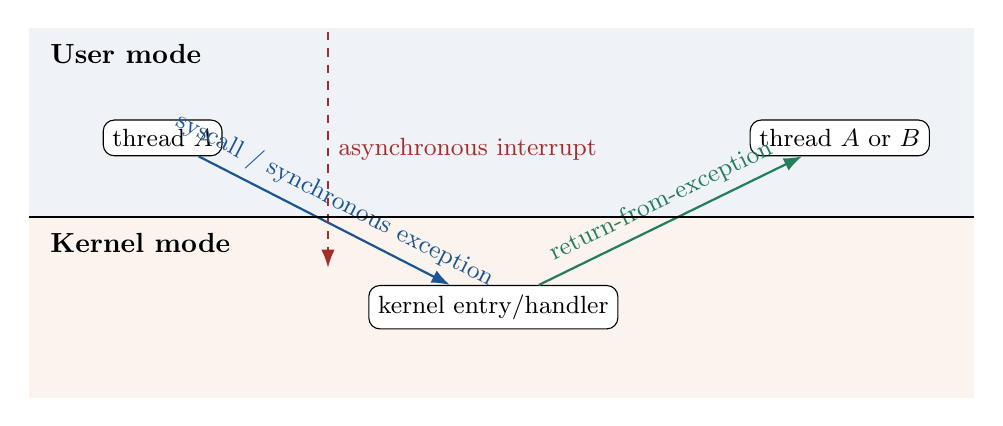
\begin{tikzpicture}[x=1cm,y=1cm,font=\small,>=Latex]
    \fill[osblue!7] (0,2.15) rectangle (12,4.55);
    \fill[osorange!8] (0,-.15) rectangle (12,2.15);
    \node[anchor=west,font=\bfseries] at (.15,4.22) {User mode};
    \node[anchor=west,font=\bfseries] at (.15,1.82) {Kernel mode};
    \node[draw,rounded corners,fill=white] (u) at (1.7,3.15) {thread $A$};
    \node[draw,rounded corners,fill=white] (k) at (5.9,1.0) {kernel entry/handler};
    \node[draw,rounded corners,fill=white] (ret) at (10.3,3.15) {thread $A$ or $B$};
    \draw[->,thick,osblue] (u)--node[above,sloped]{syscall / synchronous exception}(k);
    \draw[->,thick,dashed,osred] (3.8,4.5)--node[right]{asynchronous interrupt}(3.8,1.5);
    \draw[->,thick,osgreen] (k)--node[above,sloped]{return-from-exception}(ret);
    \draw[thick] (0,2.15)--(12,2.15);
  \end{tikzpicture}
  \begin{itemize}
    \item Hardware saves a defined entry state and transfers to a registered kernel entry path.
    \item Kernel code determines whether the current thread can resume, must block, or should be preempted.
    \item Return restores an execution context and privilege level appropriate to the selected destination.
  \end{itemize}
\end{frame}

\begin{frame}{When is the scheduler considered?}
  Common scheduling points include:
  \begin{columns}[T,onlytextwidth]
    \column{0.49\textwidth}
      \textbf{Voluntary/blocking paths}
      \begin{itemize}
        \item waiting for I/O, a lock, or an event;
        \item sleeping until a timer/deadline;
        \item explicit yield;
        \item termination.
      \end{itemize}
    \column{0.47\textwidth}
      \textbf{Preemptive/wakeup paths}
      \begin{itemize}
        \item quantum or policy accounting expires;
        \item a higher-priority thread becomes runnable;
        \item load balancing requests migration;
        \item returning from interrupt/syscall with reschedule pending.
      \end{itemize}
  \end{columns}
  \begin{tcolorbox}[title=Kernel execution is not a paradox]
    Scheduler code runs because an entry path or current kernel path already has CPU control. Kernel threads are schedulable tasks; ordinary scheduler functions are code executed in the current kernel context.
  \end{tcolorbox}
  \note{The scheduler does not need another scheduler. Some architectures and kernels defer actual rescheduling until a safe preemption point because locks, interrupt state, or invariants temporarily forbid switching.}
\end{frame}

\begin{frame}{Conceptual scheduling and dispatch path}
  \centering
  \resizebox{.96\textwidth}{!}{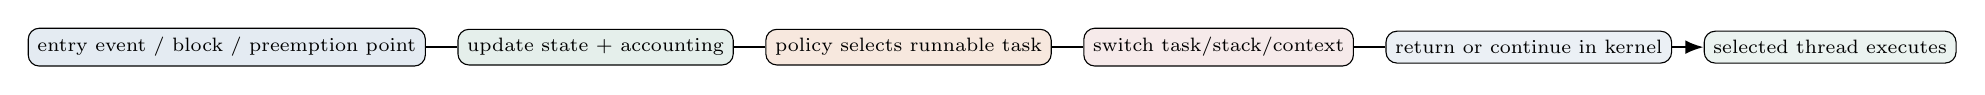
\begin{tikzpicture}[>=Latex,font=\scriptsize,node distance=4mm,every node/.style={align=center}]
    \node[draw,rounded corners,fill=osblue!12] (event) {entry event / block / preemption point};
    \node[draw,rounded corners,fill=osgreen!12,right=of event] (acct) {update state + accounting};
    \node[draw,rounded corners,fill=osorange!15,right=of acct] (pick) {policy selects runnable task};
    \node[draw,rounded corners,fill=osred!10,right=of pick] (switch) {switch task/stack/context};
    \node[draw,rounded corners,fill=osblue!9,right=of switch] (ret) {return or continue in kernel};
    \node[draw,rounded corners,fill=osgreen!9,right=of ret] (run) {selected thread executes};
    \draw[->,thick] (event)--(acct)--(pick)--(switch)--(ret)--(run);
  \end{tikzpicture}}
  \begin{itemize}
    \item If policy reselects the current thread, the expensive task-switch stage may be skipped.
    \item The selected thread can resume inside a kernel path before later returning to user mode.
    \item On multicore systems, enqueue/wakeup and eventual execution may occur on different CPUs.
  \end{itemize}
\end{frame}

% =============================================================================
\section{What a Context Switch Changes}
% =============================================================================

\begin{frame}{Context is layered, not one flat PCB snapshot}
  \scriptsize
  \begin{tabularx}{\textwidth}{@{}lXX@{}}
    \toprule
    \textbf{Layer} & \textbf{Potential state} & \textbf{When changed} \\
    \midrule
    architectural & PC, SP, flags, general registers & every switched execution stream as ABI requires \\
    extended CPU & FP/vector, matrix, debug, protection keys & eager/lazy/conditional policy \\
    kernel execution & kernel stack, current-task pointer, preemption/lock context & task handoff \\
    memory translation & page-table root, ASID/PCID, protection context & address-space change \\
    scheduler & run-queue links, runtime, class/priority, affinity & scheduling/accounting paths \\
    shared process state & files, mappings, credentials, signals & normally referenced, not copied on every switch \\
    microarchitecture & caches, TLB entries, predictors, prefetch state & affected indirectly; not normally saved/restored \\
    \bottomrule
  \end{tabularx}
  \begin{alertblock}{Correction}
    Open descriptors, PID, and most resource metadata are not loaded into CPU registers during dispatch. They remain kernel objects referenced by the selected task/process.
  \end{alertblock}
\end{frame}

\begin{frame}{Low-level handoff: a conceptual timeline}
  \centering
  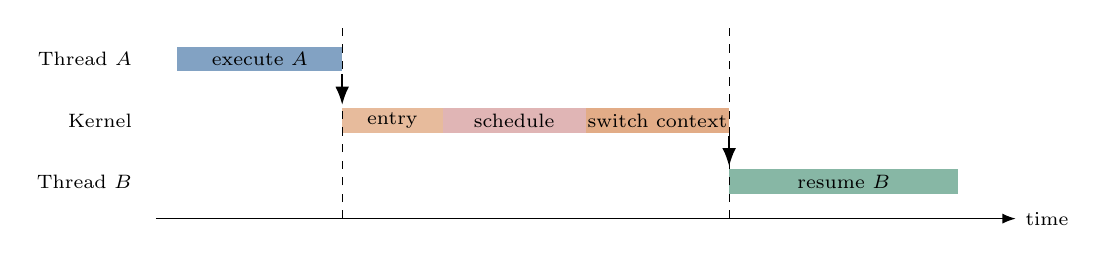
\begin{tikzpicture}[x=.91cm,y=.78cm,font=\scriptsize,>=Latex]
    \node[anchor=east] at (0,3) {Thread $A$};
    \node[anchor=east] at (0,2) {Kernel};
    \node[anchor=east] at (0,1) {Thread $B$};
    \draw[->] (.2,.4)--(12.2,.4) node[right]{time};
    \fill[osblue!55] (.5,2.8) rectangle (2.8,3.2); \node at (1.65,3) {execute $A$};
    \fill[osorange!45] (2.8,1.8) rectangle (4.2,2.2); \node at (3.5,2) {entry};
    \fill[osred!35] (4.2,1.8) rectangle (6.2,2.2); \node at (5.2,2) {schedule};
    \fill[osorange!55] (6.2,1.8) rectangle (8.2,2.2); \node at (7.2,2) {switch context};
    \fill[osgreen!55] (8.2,.8) rectangle (11.4,1.2); \node at (9.8,1) {resume $B$};
    \draw[dashed] (2.8,.4)--(2.8,3.5); \draw[dashed] (8.2,.4)--(8.2,3.5);
    \draw[->,thick] (2.8,2.75)--(2.8,2.25); \draw[->,thick] (8.2,1.75)--(8.2,1.25);
  \end{tikzpicture}
  \begin{enumerate}
    \item Preserve $A$'s resumable state and record why it stopped.
    \item Select $B$ and update run-queue/accounting state.
    \item Change kernel stack/current-task and address-space context if required.
    \item Restore $B$'s state and continue at its saved kernel/user return path.
  \end{enumerate}
  \note{The switch is often implemented by a small architecture-specific routine surrounded by scheduler code. The exact set of registers saved by hardware, compiler calling convention, and switch assembly differs.}
\end{frame}

\begin{frame}{Three handoffs with different costs}
  \begin{columns}[T,onlytextwidth]
    \column{0.31\textwidth}
      \begin{block}{Same thread}
        syscall/interrupt enters kernel and returns to the same thread.\\[.4em]
        \textbf{No scheduler task switch required.}
      \end{block}
    \column{0.31\textwidth}
      \begin{block}{Sibling threads}
        switch between threads sharing an address space.\\[.4em]
        \textbf{Stacks/registers change; mappings may remain.}
      \end{block}
    \column{0.31\textwidth}
      \begin{block}{Different processes}
        thread and address-space context may change.\\[.4em]
        \textbf{Translation/security and cache effects can grow.}
      \end{block}
  \end{columns}
  \begin{tcolorbox}[title=But do not rank blindly]
    A migrated sibling thread with a cold working set can cost more than a same-CPU process switch whose translations are tagged and whose cache footprint is small.
  \end{tcolorbox}
\end{frame}

\begin{frame}{Address-space switching, TLBs, and tagged translations}
  \begin{columns}[T,onlytextwidth]
    \column{0.51\textwidth}
      \begin{itemize}
        \item Page-table context tells the MMU how to translate virtual addresses.
        \item ASIDs/PCIDs tag translations by address space so entries can coexist in the TLB.
        \item Switching the page-table root need not flush every translation.
        \item Mapping changes still require targeted invalidation and cross-CPU TLB shootdowns.
        \item Kernel/user page-table isolation and security mitigations can add entry/switch work.
      \end{itemize}
    \column{0.45\textwidth}
      \begin{alertblock}{Indirect penalty}
        Even without a full TLB flush, the selected task can suffer capacity/conflict misses and page-table walks because another workload displaced useful entries.
      \end{alertblock}
      \begin{tcolorbox}[title=Multicore detail]
        A mapping update may interrupt other CPUs using that address space so stale translations are invalidated safely.
      \end{tcolorbox}
  \end{columns}
\end{frame}

\begin{frame}{Extended CPU state: vectors, matrices, and security}
  \begin{itemize}
    \item Modern extended register files can be large: floating-point, SIMD/vector, matrix/tile, debug, and control state.
    \item \concept{Eager switching} saves/restores state predictably but may move unused data.
    \item \concept{Lazy switching} defers restoration until first use, reducing some work but complicating faults, ownership, and security.
    \item Kernels may track which features a thread used and save variable-sized state selectively.
    \item Real-time systems often prefer predictable eager behavior over average-case optimization.
  \end{itemize}
  \begin{alertblock}{Security history lesson}
    Lazy state management can create information-leak hazards if ownership and speculation are not handled correctly. Optimization policy must preserve isolation.
  \end{alertblock}
  \note{Do not claim every register is saved on every switch. Some state is preserved by calling conventions in kernel stacks, some by explicit switch code, and some only when used. Specific policies evolve with CPU features and vulnerabilities.}
\end{frame}

\begin{frame}{Microarchitectural state is not restored like registers}
  \begin{columns}[T,onlytextwidth]
    \column{0.48\textwidth}
      \textbf{Potentially disrupted}
      \begin{itemize}
        \item private/shared cache contents;
        \item TLB and paging-structure caches;
        \item branch predictors;
        \item hardware prefetch streams;
        \item memory-controller and interconnect queues.
      \end{itemize}
    \column{0.48\textwidth}
      \textbf{Consequences}
      \begin{itemize}
        \item slower initial execution after dispatch;
        \item interference among co-runners;
        \item side channels across protection domains;
        \item high variance despite similar direct switch time.
      \end{itemize}
  \end{columns}
  \begin{tcolorbox}[title=Working-set principle]
    The indirect cost depends on the outgoing and incoming working sets, cache topology, CPU placement, and time since the incoming task last ran.
  \end{tcolorbox}
\end{frame}

% =============================================================================
\section{Preemption, Interrupts, and Kernel Execution}
% =============================================================================

\begin{frame}{Preemption requires a safe point}
  \begin{columns}[T,onlytextwidth]
    \column{0.50\textwidth}
      The kernel may temporarily defer preemption while:
      \begin{itemize}
        \item holding a spinlock or manipulating CPU-local invariants;
        \item executing hard-interrupt context;
        \item interrupts or preemption are explicitly disabled;
        \item architecture entry/exit state is incomplete;
        \item a non-preemptible critical section is active.
      \end{itemize}
    \column{0.46\textwidth}
      \begin{tcolorbox}[title=Reschedule request]
        A timer or wakeup can mark that rescheduling is needed. The actual switch occurs when execution reaches a legal scheduling point.
      \end{tcolorbox}
      \begin{alertblock}{Latency implication}
        Long non-preemptible regions, interrupt masking, or high-priority handlers can delay a ready high-priority task.
      \end{alertblock}
  \end{columns}
\end{frame}

\begin{frame}{Interrupt work is split to control latency}
  \centering
  \resizebox{.94\textwidth}{!}{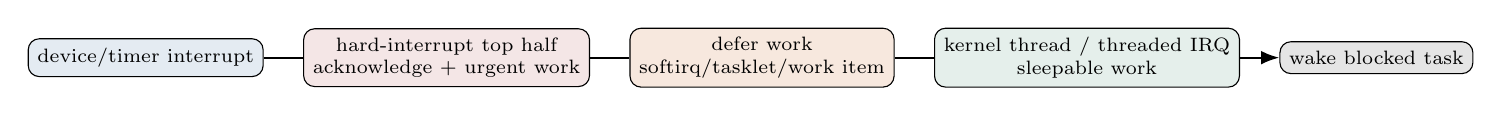
\begin{tikzpicture}[>=Latex,font=\scriptsize,node distance=5mm,every node/.style={align=center}]
    \node[draw,rounded corners,fill=osblue!12] (dev) {device/timer interrupt};
    \node[draw,rounded corners,fill=osred!12,right=of dev] (top) {hard-interrupt top half\\acknowledge + urgent work};
    \node[draw,rounded corners,fill=osorange!15,right=of top] (defer) {defer work\\softirq/tasklet/work item};
    \node[draw,rounded corners,fill=osgreen!12,right=of defer] (thread) {kernel thread / threaded IRQ\\sleepable work};
    \node[draw,rounded corners,fill=black!10,right=of thread] (wake) {wake blocked task};
    \draw[->,thick] (dev)--(top)--(defer)--(thread)--(wake);
  \end{tikzpicture}}
  \begin{itemize}
    \item Keep hard-interrupt handling bounded because it delays other interrupt and scheduling work.
    \item Deferred mechanisms differ in whether they can sleep, their priority, CPU affinity, and concurrency.
    \item Real-time configurations often thread more interrupt work so it can be prioritized and preempted.
  \end{itemize}
\end{frame}

\begin{frame}{Timer interrupts enable accounting, not automatic fairness}
  \begin{enumerate}
    \item A hardware timer event causes a privileged interrupt entry.
    \item Kernel timekeeping and scheduler accounting update elapsed runtime/timers.
    \item Policy may mark the current task for preemption or wake timed sleepers.
    \item At a valid scheduling point, the scheduler can choose a runnable task.
  \end{enumerate}
  \begin{alertblock}{No guarantee from the timer alone}
    Fairness and responsiveness depend on scheduling policy, priority configuration, runnable load, non-preemptible latency, and resource contention. Timer ticks merely provide one control mechanism.
  \end{alertblock}
  \begin{tcolorbox}[title=Tickless kernels]
    Modern kernels can program one-shot timers and suppress periodic ticks when possible. Preemption does not require a fixed global tick interval.
  \end{tcolorbox}
\end{frame}

\begin{frame}{Kernel preemption models}
  \small
  \begin{tabularx}{\textwidth}{@{}lXX@{}}
    \toprule
    \textbf{Model} & \textbf{Behavior} & \textbf{Trade-off} \\
    \midrule
    non-preemptive kernel & switch mainly on return/block/explicit points & simple invariants; potentially long latency \\
    voluntary preemption & explicit checks in long paths & improved latency; coverage depends on check placement \\
    preemptible kernel & most process-context kernel code preemptible outside protected regions & lower latency; more synchronization complexity \\
    real-time/preempt-RT style & thread interrupt/lock paths where feasible; priority-aware locking & more deterministic latency; overhead and integration constraints \\
    \bottomrule
  \end{tabularx}
  \begin{tcolorbox}[title=Design goal]
    Bound the longest interval during which a higher-priority ready task cannot execute, not merely the average context-switch instruction count.
  \end{tcolorbox}
\end{frame}

% =============================================================================
\section{Latency Decomposition and Performance}
% =============================================================================

\begin{frame}{Latency terms: define the interval before measuring}
  \centering
  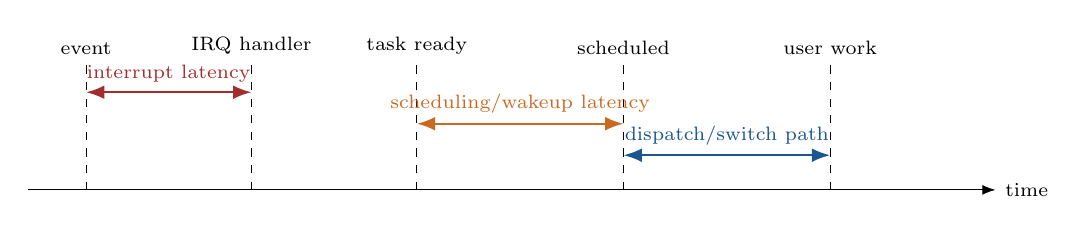
\begin{tikzpicture}[x=1.05cm,y=.8cm,font=\scriptsize,>=Latex]
    \draw[->] (.3,.5)--(12,.5) node[right]{time};
    \foreach \x/\lab in {1/{event},3/{IRQ handler},5/{task ready},7.5/{scheduled},10/{user work}} {
      \draw[dashed] (\x,.5)--(\x,2.5); \node[above,align=center] at (\x,2.5) {\lab};
    }
    \draw[<->,thick,osred] (1,2.05)--node[above]{interrupt latency}(3,2.05);
    \draw[<->,thick,osorange] (5,1.55)--node[above]{scheduling/wakeup latency}(7.5,1.55);
    \draw[<->,thick,osblue] (7.5,1.05)--node[above]{dispatch/switch path}(10,1.05);
  \end{tikzpicture}
  \begin{itemize}
    \item \concept{Interrupt latency}: event to beginning of its handler, under a stated definition.
    \item \concept{Wakeup-to-run latency}: runnable transition to execution on a CPU.
    \item \concept{Dispatch latency}: scheduling decision/dispatch point to selected execution; definitions vary.
    \item \concept{Response time}: workload-level release/request to first response or completion, depending on field.
  \end{itemize}
  \note{Many textbooks define dispatch latency as stop-one/start-another, but tools and real-time literature use more precise intervals. Require students to draw timestamp endpoints before comparing numbers.}
\end{frame}

\begin{frame}{Direct and indirect switch cost}
  A first-order decomposition is
  \[
    T_{\text{handoff}} = T_{\text{entry}} + T_{\text{scheduler}} + T_{\text{switch}}
    + T_{\text{return}} + T_{\text{warmup}}.
  \]
  \begin{columns}[T,onlytextwidth]
    \column{0.48\textwidth}
      \textbf{Direct/measured in kernel path}
      \begin{itemize}
        \item entry and accounting;
        \item run-queue selection/locking;
        \item architectural state handoff;
        \item return/mitigation work.
      \end{itemize}
    \column{0.48\textwidth}
      \textbf{Indirect/workload-visible}
      \begin{itemize}
        \item cache/TLB/predictor warmup;
        \item migration and NUMA access;
        \item queueing before dispatch;
        \item interference from co-runners.
      \end{itemize}
  \end{columns}
  \smallnote{The terms overlap depending on instrumentation; the equation is a reasoning framework, not a hardware identity.}
\end{frame}

\begin{frame}{Time quantum: overhead versus response}
  Suppose useful execution lasts quantum $q$ and a handoff costs $s$. Under a simple saturated round-robin model:
  \[
    \eta_{\text{direct}} \approx \frac{q}{q+s},
    \qquad
    f_{\text{switch}} \approx \frac{1}{q+s}.
  \]
  \begin{columns}[T,onlytextwidth]
    \column{0.49\textwidth}
      Smaller $q$ can:
      \begin{itemize}
        \item reduce worst-case turn waiting;
        \item improve interactive sharing;
        \item increase switch/cache overhead;
        \item fragment CPU bursts.
      \end{itemize}
    \column{0.47\textwidth}
      Larger $q$ can:
      \begin{itemize}
        \item improve locality/throughput;
        \item approach FCFS behavior;
        \item increase response delay under load;
        \item let latency-sensitive work wait longer.
      \end{itemize}
  \end{columns}
  \note{This model assumes one switch per full quantum and ignores blocking, multiple CPUs, scheduler policy, and indirect costs. It is useful for sensitivity analysis only. Modern schedulers may use target latency, weighted virtual runtime, or deadline parameters rather than one fixed global quantum.}
\end{frame}

\begin{frame}{Example: direct overhead is nonlinear in the quantum}
  Let $s=6\,\mu\mathrm{s}$.
  \begin{center}
  \begin{tabular}{@{}rrr@{}}
    \toprule
    $q$ & overhead $s/(q+s)$ & useful efficiency $q/(q+s)$ \\
    \midrule
    $20\,\mathrm{ms}$ & $0.030\%$ & $99.970\%$ \\
    $1\,\mathrm{ms}$ & $0.596\%$ & $99.404\%$ \\
    $100\,\mu\mathrm{s}$ & $5.66\%$ & $94.34\%$ \\
    \bottomrule
  \end{tabular}
  \end{center}
  \begin{alertblock}{Interpret carefully}
    These percentages cover only the assumed direct $6\,\mu\mathrm{s}$ cost. Cache/TLB disruption, migration, queueing, and shortened useful bursts may dominate.
  \end{alertblock}
\end{frame}

\begin{frame}{Tail latency matters more than the average}
  \begin{columns}[T,onlytextwidth]
    \column{0.49\textwidth}
      Sources of long tails:
      \begin{itemize}
        \item interrupt storms or long handlers;
        \item lock contention and priority inversion;
        \item CPU frequency/idle-state exit;
        \item NUMA migration and cache misses;
        \item page faults, reclaim, and write-back;
        \item virtualization steal time.
      \end{itemize}
    \column{0.47\textwidth}
      \begin{tcolorbox}[title=Report distributions]
        Measure median, high percentiles, maximum under a defined test window, and outliers with causal traces. A low mean does not establish a real-time bound.
      \end{tcolorbox}
      \begin{alertblock}{Coordinated omission}
        A load generator that pauses during stalls can underreport exactly the latency experienced by a fixed-rate workload.
      \end{alertblock}
  \end{columns}
\end{frame}

\begin{frame}{Real-time focus: bounded interference}
  A high-priority task's release-to-run latency can include:
  \[
    L \leq B_{\text{irq-off}} + B_{\text{nonpreempt}}
      + B_{\text{lock}} + I_{\text{higher-priority}} + C_{\text{dispatch}},
  \]
  under an explicit analysis model.
  \begin{itemize}
    \item $B$ terms bound interrupt masking, non-preemptible regions, and resource blocking.
    \item $I$ captures interference from work allowed to outrank the task.
    \item $C_{\text{dispatch}}$ includes the relevant scheduler/switch path.
  \end{itemize}
  \begin{alertblock}{Not a complete theorem}
    Hardware contention, DMA, cache effects, firmware/system-management interrupts, release jitter, and multicore interference must be modeled or controlled for a defensible bound.
  \end{alertblock}
\end{frame}

% =============================================================================
\section{Multicore Dispatch and System Load}
% =============================================================================

\begin{frame}{Per-CPU run queues and wakeup placement}
  \centering
  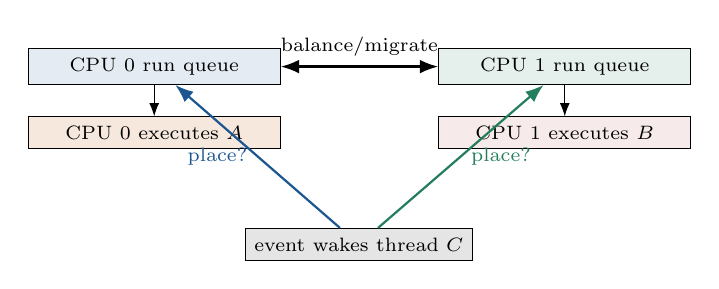
\begin{tikzpicture}[>=Latex,font=\scriptsize,node distance=4mm,every node/.style={align=center}]
    \node[draw,fill=osblue!12,minimum width=3.2cm] (r0) {CPU 0 run queue};
    \node[draw,fill=osgreen!12,minimum width=3.2cm,right=2cm of r0] (r1) {CPU 1 run queue};
    \node[draw,fill=osorange!15,minimum width=3.2cm,below=of r0] (c0) {CPU 0 executes $A$};
    \node[draw,fill=osred!10,minimum width=3.2cm,below=of r1] (c1) {CPU 1 executes $B$};
    \node[draw,fill=black!10,below=1cm of c0,xshift=2.6cm] (w) {event wakes thread $C$};
    \draw[->] (r0)--(c0); \draw[->] (r1)--(c1);
    \draw[<->,thick] (r0)--node[above]{balance/migrate}(r1);
    \draw[->,thick,osblue] (w)--node[left]{place?}(r0);
    \draw[->,thick,osgreen] (w)--node[right]{place?}(r1);
  \end{tikzpicture}
  \begin{itemize}
    \item Per-CPU queues reduce global locking but create imbalance and placement decisions.
    \item Wakeup policy considers idle CPUs, previous CPU/cache affinity, NUMA, priority, energy, and capacity.
    \item Cross-CPU wakeups may require inter-processor interrupts; migration can disturb locality.
  \end{itemize}
\end{frame}

\begin{frame}{Heterogeneous CPUs and capacity-aware dispatch}
  \begin{columns}[T,onlytextwidth]
    \column{0.50\textwidth}
      Modern systems may combine cores with different:
      \begin{itemize}
        \item peak performance and energy efficiency;
        \item vector/matrix capability or frequency range;
        \item cache topology and memory proximity;
        \item thermal headroom and current load.
      \end{itemize}
    \column{0.46\textwidth}
      \begin{tcolorbox}[title=Policy problem]
        Place latency-critical or compute-heavy tasks on sufficient-capacity CPUs while preserving energy efficiency and avoiding migrations.
      \end{tcolorbox}
      \begin{alertblock}{Observation}
        ``CPU utilization'' does not capture whether work ran on an appropriate-capacity core or was throttled by power/thermal policy.
      \end{alertblock}
  \end{columns}
\end{frame}

\begin{frame}{Degree of multiprogramming: modern interpretation}
  The historical term means how many jobs/processes are admitted into active competition. On modern systems, separate:
  \begin{itemize}
    \item \concept{runnable load}: tasks competing for CPU capacity;
    \item \concept{memory working sets}: active pages competing for RAM/cache/TLB capacity;
    \item \concept{blocked concurrency}: tasks waiting on I/O, locks, or remote services;
    \item \concept{resource-control admission}: cgroups, quotas, pools, and service limits;
    \item \concept{in-flight requests}: application concurrency and queue depth.
  \end{itemize}
  \begin{alertblock}{Correction}
    More resident processes do not directly imply more context switches. Switching frequency depends on runnable tasks, blocking/wakeup behavior, quantum/policy, CPU count, and synchronization.
  \end{alertblock}
\end{frame}

\begin{frame}{Queueing explains why excess concurrency hurts latency}
  Little's law for a stable system relates average in-flight work $N$, throughput $\lambda$, and average time $W$:
  \[
    N = \lambda W.
  \]
  \begin{columns}[T,onlytextwidth]
    \column{0.49\textwidth}
      Increasing concurrency can initially:
      \begin{itemize}
        \item hide I/O latency;
        \item keep CPUs/devices utilized;
        \item raise throughput toward capacity.
      \end{itemize}
    \column{0.47\textwidth}
      Beyond bottleneck capacity it often:
      \begin{itemize}
        \item grows queues and tail latency;
        \item increases cache and lock contention;
        \item amplifies memory pressure;
        \item adds work without throughput gain.
      \end{itemize}
  \end{columns}
  \note{Little's law is an identity for long-run stable averages under broad conditions, not a prescription that more concurrency creates throughput. Once arrival rate exceeds sustainable service rate, queues grow without a finite steady-state W.}
\end{frame}

\begin{frame}{Thrashing is a working-set failure, not switch overhead}
  \begin{columns}[T,onlytextwidth]
    \column{0.50\textwidth}
      \concept{Thrashing} occurs when active memory demand exceeds available capacity so page faults/reclaim dominate useful work.
      \begin{itemize}
        \item major faults can wait on storage;
        \item reclaim/write-back consumes CPU and I/O;
        \item tasks repeatedly evict each other's useful pages;
        \item adding work can reduce throughput.
      \end{itemize}
    \column{0.46\textwidth}
      \begin{alertblock}{Context switches are secondary}
        Faults block and wake tasks, so switching may rise, but the root problem is insufficient memory for active working sets and poor admission/control.
      \end{alertblock}
      \begin{tcolorbox}[title=Mitigation]
        Reduce concurrency, enforce memory limits, improve locality, add memory, tune reclaim, or redesign the workload/data path.
      \end{tcolorbox}
  \end{columns}
\end{frame}

% =============================================================================
\section{Implementation and Observability}
% =============================================================================

\begin{frame}{Linux: useful implementation landmarks}
  \begin{columns}[T,onlytextwidth]
    \column{0.51\textwidth}
      \begin{itemize}
        \item schedulable entities are represented by per-thread task records with shared process objects;
        \item scheduler classes implement different policies over per-CPU run queues;
        \item a low-level architecture-specific switch changes task/stack and required machine state;
        \item wakeups, balancing, affinity, cgroups, and NUMA influence placement;
        \item preemption configuration changes where kernel execution can be displaced.
      \end{itemize}
    \column{0.45\textwidth}
      \begin{alertblock}{Avoid stale slogans}
        Linux is not accurately summarized as ``CFS uses a red-black tree'' for every task and kernel version. Multiple scheduler classes and evolving fair-scheduler implementations coexist.
      \end{alertblock}
      \begin{tcolorbox}[title=Stable lesson]
        Separate policy/class logic from the architecture-specific handoff and from shared task/process state.
      \end{tcolorbox}
  \end{columns}
  \note{Implementation details change. Teach interfaces and invariants first, then have students inspect the source for the course kernel version. Do not call task_struct simply a one-per-process PCB; it is per task/thread.}
\end{frame}

\begin{frame}{Windows: analogous concepts, different organization}
  \begin{itemize}
    \item Threads are dispatchable execution entities; processes supply address-space and resource context.
    \item Priority-driven preemptive scheduling uses per-processor and system coordination structures.
    \item Deferred Procedure Calls and interrupt request levels defer/order kernel work under Windows-specific rules.
    \item Context switching and trap handling include architecture-specific state plus kernel dispatcher bookkeeping.
    \item Processor groups, affinity, heterogeneous scheduling, and power management affect placement on modern systems.
  \end{itemize}
  \begin{tcolorbox}[title=Comparison discipline]
    Compare observable semantics and concrete paths rather than forcing Linux names such as run queue or softirq onto Windows internals.
  \end{tcolorbox}
\end{frame}

\begin{frame}{Virtualization adds another scheduling layer}
  \centering
  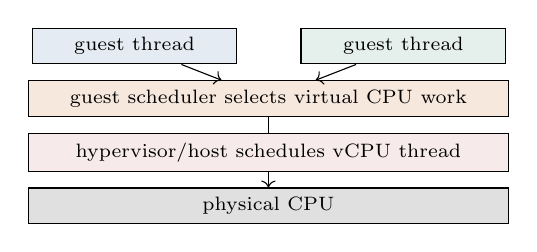
\begin{tikzpicture}[font=\scriptsize,node distance=2mm,every node/.style={align=center}]
    \node[draw,fill=osblue!12,minimum width=2.6cm] (g1) {guest thread};
    \node[draw,fill=osgreen!12,minimum width=2.6cm,right=8mm of g1] (g2) {guest thread};
    \node[draw,fill=osorange!15,minimum width=6.1cm,below=of g1,xshift=1.7cm] (gs) {guest scheduler selects virtual CPU work};
    \node[draw,fill=osred!10,minimum width=6.1cm,below=of gs] (hv) {hypervisor/host schedules vCPU thread};
    \node[draw,fill=black!12,minimum width=6.1cm,below=of hv] (pcpu) {physical CPU};
    \draw[->] (g1)--(gs); \draw[->] (g2)--(gs); \draw[->] (gs)--(hv)--(pcpu);
  \end{tikzpicture}
  \begin{itemize}
    \item A guest can schedule a thread onto a vCPU that the host is not currently running.
    \item Oversubscription, vCPU preemption, interrupt virtualization, and lock-holder preemption add latency variance.
    \item Guest CPU utilization can hide host ``steal'' time or placement problems.
  \end{itemize}
\end{frame}

\begin{frame}[fragile]{Observe counters first, then trace causality}
\begin{lstlisting}[language=bash]
# Per-thread snapshots and switch rates
ps -eLo pid,tid,psr,stat,ni,rtprio,comm
pidstat -w -t 1

# Aggregate counters for a workload
perf stat -e context-switches,cpu-migrations,page-faults -- ./workload

# Scheduler events for causal timing (permissions may be required)
perf sched record -- ./workload
perf sched timehist
\end{lstlisting}
  \begin{alertblock}{Interpretation rule}
    A high switch count can be healthy asynchronous concurrency or pathological contention. Determine who blocked, who woke it, runnable delay, CPU migration, and the work completed per switch.
  \end{alertblock}
\end{frame}

\begin{frame}{Microbenchmark pitfalls}
  \begin{columns}[T,onlytextwidth]
    \column{0.49\textwidth}
      A useful switch benchmark must control:
      \begin{itemize}
        \item same CPU versus migration;
        \item sibling threads versus processes;
        \item warm versus cold working sets;
        \item CPU frequency and idle states;
        \item competing interrupts/tasks;
        \item clock source and measurement overhead.
      \end{itemize}
    \column{0.47\textwidth}
      \begin{alertblock}{Do not use \code{sched\_yield()} as a universal switch timer}
        Yield semantics depend on policy and runnable competitors; the caller can be selected again, and the result mixes scheduler policy with switch cost.
      \end{alertblock}
      \begin{tcolorbox}[title=Report]
        Full distribution, topology, affinity, task relationship, kernel configuration, mitigations, and source code.
      \end{tcolorbox}
  \end{columns}
\end{frame}

\begin{frame}{Off-CPU analysis finds where threads actually wait}
  \begin{itemize}
    \item On-CPU profiles show instructions consuming CPU time.
    \item Off-CPU traces attribute blocked intervals to locks, I/O, timers, paging, or scheduler delay.
    \item Wakeup-to-run traces separate ``event completed'' from ``thread received a CPU.''
    \item CPU-migration and cache-counter correlation can expose locality losses.
    \item Pressure-stall information distinguishes CPU, memory, and I/O contention at system/cgroup scope.
  \end{itemize}
  \begin{tcolorbox}[title=Diagnostic sequence]
    Identify the latency interval, find its queue, determine the wakeup event, measure runnable delay, and then inspect dispatch/warmup cost.
  \end{tcolorbox}
\end{frame}

% =============================================================================
\section{Synthesis}
% =============================================================================

\begin{frame}{End-to-end preemption example}
  \centering
  \resizebox{.96\textwidth}{!}{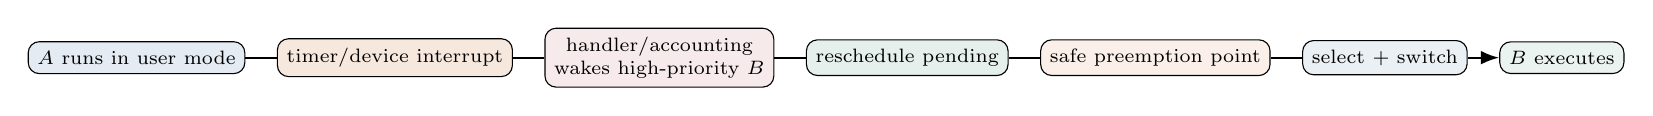
\begin{tikzpicture}[>=Latex,font=\scriptsize,node distance=4mm,every node/.style={align=center}]
    \node[draw,rounded corners,fill=osblue!12] (a) {$A$ runs in user mode};
    \node[draw,rounded corners,fill=osorange!15,right=of a] (irq) {timer/device interrupt};
    \node[draw,rounded corners,fill=osred!10,right=of irq] (work) {handler/accounting\\wakes high-priority $B$};
    \node[draw,rounded corners,fill=osgreen!12,right=of work] (mark) {reschedule pending};
    \node[draw,rounded corners,fill=osorange!10,right=of mark] (safe) {safe preemption point};
    \node[draw,rounded corners,fill=osblue!9,right=of safe] (sw) {select + switch};
    \node[draw,rounded corners,fill=osgreen!9,right=of sw] (b) {$B$ executes};
    \draw[->,thick] (a)--(irq)--(work)--(mark)--(safe)--(sw)--(b);
  \end{tikzpicture}}
  \begin{itemize}
    \item Interrupt arrival, task wakeup, scheduler decision, low-level handoff, and useful execution are distinct timestamps.
    \item If preemption is temporarily disabled, $B$ is runnable but cannot yet execute.
    \item Tail latency may be dominated by handler work, locks, CPU placement, or cache warmup rather than register save/restore.
  \end{itemize}
\end{frame}

\begin{frame}{Misconceptions corrected}
  \scriptsize
  \begin{tabularx}{\textwidth}{@{}X@{\quad$\Rightarrow$\quad}X@{}}
    \toprule
    \textbf{Misconception} & \textbf{Precise statement} \\
    \midrule
    A context switch always follows a syscall. & Same-thread kernel entry/return needs no task switch. \\
    The dispatcher loads the whole PCB. & It changes required execution context; shared resources remain referenced objects. \\
    Every timer interrupt switches tasks. & It updates time/accounting; policy may retain the current task. \\
    All registers are saved on every switch. & State depends on architecture, ABI, usage, and eager/lazy policy. \\
    More processes directly cause more switching. & Runnable/wakeup behavior, policy, CPU count, and quantum determine switches. \\
    Thrashing is excessive context switching. & It is failure to retain active memory working sets; switching is secondary. \\
    Low average switch time means real-time safety. & Bounds require worst-case interference and non-preemptible analysis. \\
    The kernel has unrestricted direct access to all physical memory. & Kernel access follows architecture mappings, permissions, isolation, and device/IOMMU mechanisms. \\
    \bottomrule
  \end{tabularx}
\end{frame}

\begin{frame}{Key takeaways}
  \begin{itemize}
    \item Scheduling chooses; dispatch and context-switch mechanisms realize the decision.
    \item Kernel entry, mode switch, scheduler invocation, task switch, and user return are distinct events.
    \item Direct switch instructions are only part of cost; working-set disruption and queueing dominate many workloads.
    \item Preemption happens only at legal points; interrupt masking, locks, and handlers determine latency tails.
    \item Multicore dispatch includes wakeup placement, balancing, affinity, NUMA, capacity, and migration.
    \item Concurrency should saturate useful resources without creating unbounded queues or memory thrashing.
    \item Measurement must define endpoints and combine counters with causal traces.
  \end{itemize}
\end{frame}

\begin{frame}{Laboratory: decompose wakeup-to-run latency}
  \begin{enumerate}
    \item Create a producer that periodically wakes a blocked worker through a pipe/eventfd.
    \item Pin both threads to one CPU, then to separate CPUs; record scheduling events.
    \item Measure event timestamp, wakeup timestamp, dispatch timestamp, and first worker instruction.
    \item Add CPU competition, memory pressure, and a migrating configuration separately.
    \item Report distributions and attribute the new delay to queueing, migration, faults, or warmup.
  \end{enumerate}
  \begin{alertblock}{Method}
    Change one factor at a time and include tracing overhead/control runs. Do not report one minimum value as system latency.
  \end{alertblock}
\end{frame}

\begin{frame}{Next week: scheduling algorithms}
  \begin{itemize}
    \item FCFS, SJF/SRTF, round robin, priority, and feedback queues;
    \item response, waiting, turnaround, throughput, fairness, and tail latency;
    \item starvation, aging, priority inversion, and admission control;
    \item schedule construction and quantitative metric comparison;
    \item linking algorithm assumptions to modern multicore implementations.
  \end{itemize}
  \begin{tcolorbox}[title=Preparation]
    For three jobs with different arrivals and CPU bursts, draw FCFS, SRTF, and round-robin schedules. State every tie-breaking assumption.
  \end{tcolorbox}
\end{frame}

% =============================================================================
\appendix
\section{Appendix}
% =============================================================================

\begin{frame}{Knowledge check: mechanism}
  \begin{enumerate}
    \item Can a mode switch occur without a context switch? Give two examples.
    \item Can a context switch occur without an immediate return to user mode?
    \item Why might sibling-thread switching preserve the address-space context?
    \item What prevents a runnable high-priority task from preempting immediately?
    \item Why can tagged TLBs reduce but not eliminate translation warmup cost?
    \item Which state is normally referenced rather than copied during dispatch?
  \end{enumerate}
  \note{Answers: (1) syscall/exception or interrupt returning to same task. (2) yes, between kernel threads or while resuming another task's kernel path. (3) shared mappings/page tables. (4) interrupt/preemption disable, locks, higher-priority work. (5) capacity/conflict misses and invalidations remain. (6) files, credentials, mappings, and other shared kernel objects.}
\end{frame}

\begin{frame}{Knowledge check: performance}
  \begin{enumerate}
    \item Distinguish interrupt latency, wakeup-to-run latency, and switch-path time.
    \item Why can same-process switching be slower than a process switch?
    \item What does a context-switch counter fail to reveal?
    \item Why does a smaller quantum eventually reduce throughput?
    \item How can CPU migration increase latency without changing direct switch code?
    \item Why is a low mean insufficient for a hard real-time claim?
  \end{enumerate}
\end{frame}

\begin{frame}{Exercise: quantum sensitivity}
  A saturated one-CPU system runs $n=8$ equal tasks under ideal round robin. Direct handoff cost is $s=5\,\mu\mathrm{s}$.
  \begin{enumerate}
    \item Compute direct efficiency for $q=10\,\mathrm{ms}$, $1\,\mathrm{ms}$, and $100\,\mu\mathrm{s}$.
    \item Estimate the maximum time before a just-missed task receives service under the ideal model.
    \item Add a $20\,\mu\mathrm{s}$ average cache-warmup penalty and recompute useful efficiency.
    \item Explain why averages cannot be added this way for a worst-case bound.
  \end{enumerate}
\end{frame}

\begin{frame}{Exercise: reconstruct the latency path}
  A high-priority thread becomes runnable at $t=10\,\mu\mathrm{s}$, but executes at $t=85\,\mu\mathrm{s}$. Trace data shows:
  \begin{itemize}
    \item interrupt handler completes at $30\,\mu\mathrm{s}$;
    \item preemption is disabled until $60\,\mu\mathrm{s}$;
    \item scheduler and handoff finish at $72\,\mu\mathrm{s}$;
    \item first cache-miss-heavy useful operation finishes at $85\,\mu\mathrm{s}$.
  \end{itemize}
  \begin{enumerate}
    \item Attribute intervals to handler, non-preemptible, switch, and warmup components.
    \item Which component should each optimization target?
    \item Which timestamps would a simple switch counter omit?
  \end{enumerate}
\end{frame}

\begin{frame}{Exercise: concurrency and queueing}
  A service completes $4{,}000$ requests/s at saturation. At 20 in-flight requests, mean latency is $5$ ms.
  \begin{enumerate}
    \item Verify consistency with Little's law.
    \item If concurrency rises to 100 with unchanged throughput, what mean latency follows in steady state?
    \item List reasons throughput may instead fall: cache pressure, locks, context switching, memory reclaim, downstream saturation.
    \item Propose an admission-control signal and a safe control objective.
  \end{enumerate}
  \note{At 4,000/s and 5 ms, N=20. With N=100 and unchanged throughput, W=25 ms. The calculation assumes stable long-run averages and does not predict percentiles.}
\end{frame}

\begin{frame}[fragile]{Optional tracing commands}
\begin{lstlisting}[language=bash]
# Per-thread switches and migrations once per second
pidstat -w -t 1

# Scheduler timeline for one command
perf sched record -- ./workload
perf sched timehist

# Counters (names/support vary by platform)
perf stat -e task-clock,context-switches,cpu-migrations,page-faults \
  -- ./workload
\end{lstlisting}
  \smallnote{Run only with appropriate permissions. Trace buffers, symbol access, and event availability vary by kernel and security policy.}
\end{frame}

\begin{frame}{Further study}
  \begin{itemize}
    \item architecture entry/switch assembly and extended-state management;
    \item preemptible kernels, PREEMPT\_RT, threaded interrupts, priority inheritance;
    \item scheduler tracepoints, off-CPU flame graphs, eBPF latency analysis;
    \item TLB shootdowns, ASIDs/PCIDs, cache partitioning, NUMA balancing;
    \item heterogeneous scheduling, energy-aware placement, thermal control;
    \item vCPU scheduling, steal time, nested virtualization, real-time guests.
  \end{itemize}
  \begin{center}
    \Large Questions?
  \end{center}
\end{frame}

\end{document}

